\chapter{Analysis}
After utilizing the AUSAlib tools, the data is ready to be analyzed. Even though the theory dictates that a decay will consist of two \al-particles and one \be-particles, it is not realistic to just assume that each detected event will consist only of this configuration of particles. \\
Therefore we need some cut on what events we will allow through to the analysis. Specifically we are going to impose 3 cuts on the data, a angular cut, a momentum cut and a multiplicity cut.

\section{Identifying the particles}
When a particle hits a given detector, we have no real knowledge of what particle it is. 
Therefore we need to do an analysis where we identify what particle we have.

This is done in \textcolor{red}{XX} steps
\subsection{Finding a hit}
The first step ind identifying a hit, is to actually get a hit, and gather the different properties of the specific hit. 

\subsection{Identifying a hit}
After a hit has been has been detected, and all the relevant information has been extracted from the hit, we can start to analyze what type of particle has hit the detector. 

A important distinction between an \al-particle and a \be-particle is the different interactions with a detector. An \al-particle will be compleatly stopped by a standard \SI{60}{\mu m} detector, while a \be-particle will pass through it, depositing only a small amount of energy. \\
This is the reason for the SSD's behind each DSSD. The idea is that only a \be-particle will be detected in the SSD's, so if a hit has some energy in a DSSD \textit{and} the corresponding SSD, it will be classified as a \be-particle.




\section{Angular cut}
When a particle hits a given detector, we have no real knowledge of what particle it is. 
Therefore we need to use other properties of the decay to determine the particle type. 
When \isotope[8][]Be decays, and produces the two \al-particles, it will do so under conservation of momentum. The decay in any direction, but the angle between $\theta$ them will be close to  $180\degree$, or $\cos(\theta) \geq -1$. Therefore the first cut that we give to the data, is that two of the particles that are \al candidates, must have a mutual angle of close to $180\degree$.\\


On \cref{fig:cosAll} a plot of all the the mutual angles are shown. A quick glance will give that most particles will have mutual angle of close to $180\degree$. 

\begin{figure}[h]
	\centering
	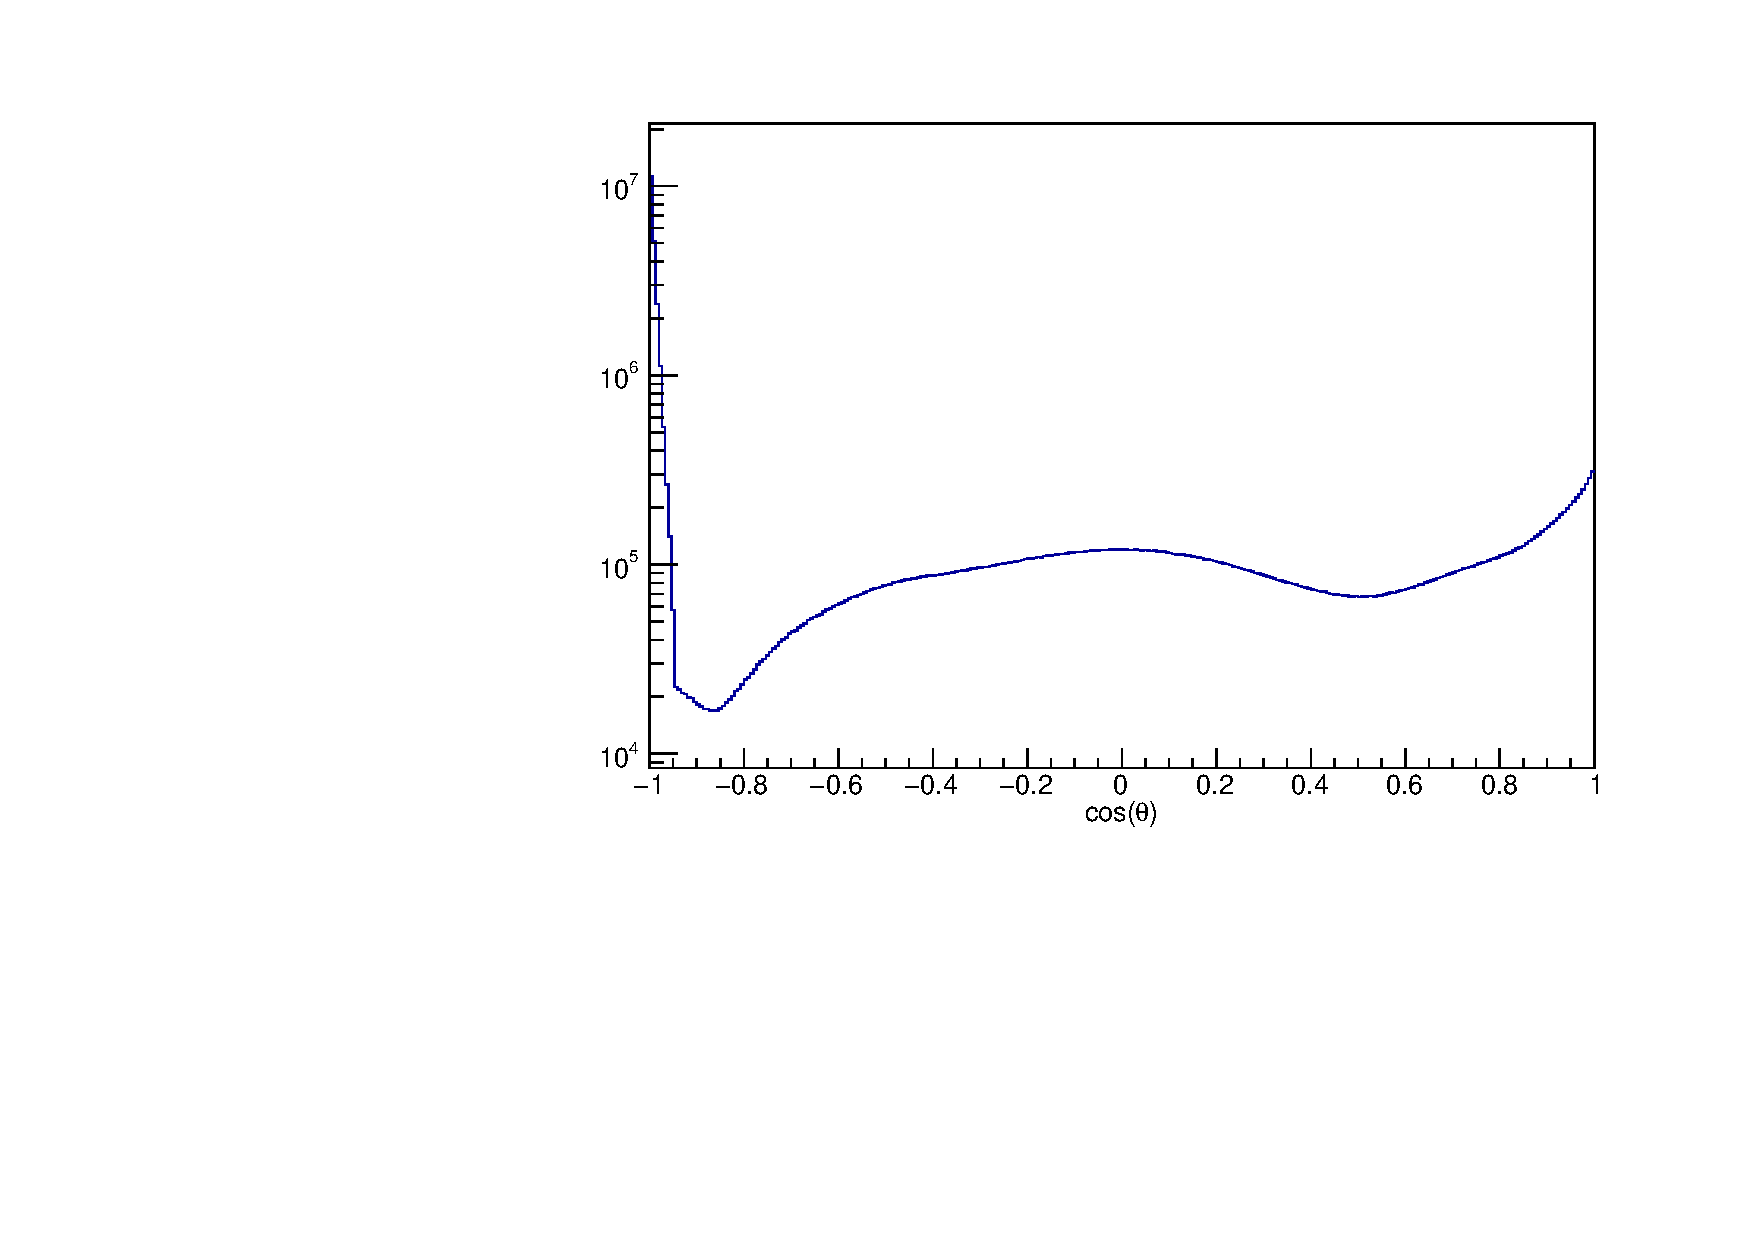
\includegraphics[width=\linewidth]{../figures/cosang.pdf}
	\caption{A histogram of all the mutual angles between all particles.}
	\label{fig:cosAll}
\end{figure}

By looking at this, we see that most of the angles will lie close to $180\degree$, and now we must decide exactly where to do the cutoff. 
By taking a sharp cutoff at $\cos(\theta) \geq -0.99$, we will exclude a great deal of good measurements, on the other hand, a too soft cut will not accomplish anything, as too many "wrong" particles will let through the check. 



\section{Momentum cut}

\section{Multiplicity cut}
The last cut that we want to impose on the data, is a multiplicity cut. This cut is just to ensure that we have the amount of particles that we expect. 
Therefore a hard criteria is that there must be at least two distinctly identified \al-particles. \\

With regards to the \be-particles, we are more loose. Here we say that there must at least be one, but more can occur. This is quite rare, but the we still take that event into account, as the \be-particles should have an isotropic distribution, and therefore should not in any case be affected by the other \al-particles. On \cref{fig:betaMul} we see the multiplicity of \be-particles, and it is quite rare that there are more than one in a given event, so most of the time there \textcolor{red}{CONTINUE HERE}